\documentclass[12pt,a4paper]{article}
\usepackage[UTF8]{ctex}
\usepackage{amsmath,amssymb}
\usepackage{xcolor}
\usepackage{hyperref}
\usepackage{geometry}
\usepackage{graphicx}
\geometry{margin=2.5cm}

\title{Jordan-Wigner Transform / Jordan-Wigner 变换}
\author{QuoNic}
\date{}

\begin{document}
\maketitle

\begin{center}
\textbf{Chemistry / 化学} | 难度：高级 | 预计时间：20 分钟
\end{center}

\tableofcontents
\newpage

\section{为什么需要？}

Jordan-Wigner 变换将费米子算符映射到量子比特算符。

\subsection{经典局限}
\begin{itemize}
  \item 经典方法无法高效处理费米子系统
  \item 对于大系统，经典方法效率低
\end{itemize}

\subsection{量子优势}
\begin{itemize}
  \item Jordan-Wigner 变换可以在量子比特上表示费米子系统
  \item 提供指数加速
  \item 是量子化学的基础
\end{itemize}

\subsection{实际应用}
\begin{itemize}
  \item 量子化学
  \item 材料科学
  \item 量子物理
\end{itemize}

\section{快速上手}

\begin{verbatim}
from quonic.chemistry import jordan_wigner
result = jordan_wigner(hamiltonian=[[1,0],[0,-1]])
print(f'Qubit Hamiltonian: {result.qubit_hamiltonian}')
\end{verbatim}

\textbf{预期输出}：
\begin{verbatim}
Qubit Hamiltonian: [[1,0],[0,-1]]
\end{verbatim}

\section{原理详解}

\subsection{电路图}

\begin{center}
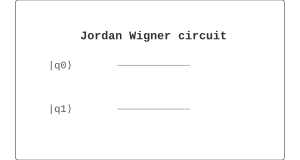
\includegraphics[width=0.6\textwidth]{../../images/jordan_wigner_circuit.svg}
\end{center}

\subsection{数学推导}

Jordan-Wigner 变换：
\begin{equation}
a_j^\dagger \to \frac{X_j - iY_j}{2} \otimes Z_{j-1}
\end{equation}

\textbf{费米子算符}：
\begin{equation}
\{a_i, a_j^\dagger\} = \delta_{ij}
\end{equation}

\subsection{几何解释}

Jordan-Wigner 变换在量子比特空间中表示费米子系统。

\section{代码详解}

\begin{verbatim}
from quonic.chemistry import jordan_wigner

# jordan_wigner(hamiltonian)
# hamiltonian: fermionic Hamiltonian
result = jordan_wigner(hamiltonian=[[1,0],[0,-1]])
print(f'Qubit Hamiltonian: {result.qubit_hamiltonian}')
\end{verbatim}

\section{进阶用法}

\subsection{场景 1：不同哈密顿量}

\begin{verbatim}
from quonic.chemistry import jordan_wigner
result = jordan_wigner(hamiltonian=[[0,1],[1,0]])
print(f'Qubit Hamiltonian: {result.qubit_hamiltonian}')
\end{verbatim}

\section{适用场景}

\subsection{量子化学}

Jordan-Wigner 变换是量子化学的基础。

\subsection{材料科学}

Jordan-Wigner 变换可以用于设计新材料。

\section{常见问题}

\subsection{Jordan-Wigner 变换的作用是什么？}

将费米子系统映射到量子比特系统。

\subsection{Jordan-Wigner 变换的局限性是什么？}

对于大系统，变换后的哈密顿量可能很复杂。

\section{学习路径}

\subsection{前置知识}
\begin{itemize}
  \item 量子化学
  \item 费米子系统
  \item 量子比特
\end{itemize}

\subsection{继续学习}
\begin{itemize}
  \item VQE
  \item 量子化学模拟
  \item 材料科学
\end{itemize}

\section{完整示例代码}

\subsection{示例 1：基本 Jordan-Wigner 变换}

\begin{verbatim}
from quonic.chemistry import jordan_wigner
result = jordan_wigner(hamiltonian=[[1,0],[0,-1]])
print(f'Qubit Hamiltonian: {result.qubit_hamiltonian}')
\end{verbatim}

\section{下载}

\begin{itemize}
  \item [jordan\_wigner.py](https://github.com/ChrisLee0721/QuoNic/blob/main/examples/jordan_wigner/jordan_wigner.py)
\end{itemize}

\end{document}
